\documentclass[sn-mathphys,pdflatex,iicol]{sn-jnl}% Math and Physical Sciences Reference Style

%%%% Standard Packages
\usepackage{polyglossia} % Must come before biblatex

\usepackage{bm}
\usepackage{csquotes}
\usepackage{fontspec}
\usepackage{hyperref}
%\usepackage{lua-visual-debug}
\usepackage{tabularx}
%%%%

\jyear{2022}

%% as per the requirement new theorem styles can be included as shown below
%%\theoremstyle{thmstyleone}%
%%\newtheorem{theorem}{Theorem}[section]% meant for sectionwise numbers
%% optional argument [theorem] produces theorem numbering sequence instead of independent numbers for Proposition
%%\newtheorem{proposition}[theorem]{Proposition}%
%%\newtheorem{proposition}{Proposition}% to get separate numbers for theorem and proposition etc.

%%\theoremstyle{thmstyletwo}%
%%\newtheorem{example}{Example}%
%%\newtheorem{remark}{Remark}%

%%\theoremstyle{thmstylethree}%
%%\newtheorem{definition}{Definition}%

\raggedbottom
%%\unnumbered% uncomment this for unnumbered level heads

\setdefaultlanguage{english}
\setotherlanguage{czech}

\hypersetup{
	pdfencoding=auto,
	unicode=true,
	bookmarksopen=true,
	bookmarksopenlevel=3
}

\newcommand{\name}[1]{\textit{#1}}
\newcommand{\mathfield}{\ensuremath{\mathbb}}
\newcommand{\mathmat}{\ensuremath{\mathbf}}
\newcommand{\mathset}{\ensuremath{\mathbb}}
\newcommand{\mathspace}{\ensuremath{\mathcal}}
\newcommand{\mathvec}{\ensuremath{\bm}}

\newcounter{enumroman}
\newenvironment{romanitems}{\begin{list}{\bfseries(\roman{enumroman})\hfill}{\usecounter{enumroman}\setlength{\labelwidth}{\leftmargin}\addtolength{\labelwidth}{-1\labelsep}\topsep=0mm plus 2pt\itemsep=0mm\parsep=0mm plus 2pt\itemindent=0mm}}{\end{list}}

\DeclareMathOperator*{\argmin}{arg\,min}
\DeclareMathOperator*{\argmax}{arg\,max}


\begin{document}

\copyrightyear{2022}
\copyrightclause{Use permitted under Creative Commons License Attribution 4.0 International (CC BY 4.0).}

\conference{Data and Model Quality for Mining and Learning with Graphs: Methods and Open Challenges
@ECML-PKDD 2022, September 23, 2022, Grenoble, France}

\title{Balancing performance and complexity in hierarchical coarsening of graphs}
\author[1,2]{Marek Dědič}[orcid=0000-0003-1021-8428,email=marek@dedic.eu,url=https://dedic.eu]
\cormark[1]
\author[2]{Lukáš Bajer}
\author[2]{Jakub Repický}
\author[2]{Pavel Procházka}
\author[3]{Martin Holeňa}

\address[1]{Czech Technical University in Prague, Břehová 7, Prague, Czech Republic}
\address[2]{Cisco Systems, Inc., Karlovo náměstı́ 10, Prague, Czech Republic}
\address[3]{Institute of Computer Science, Czech Academy of Sciences, Pod vodárenskou věží 2, Prague, Czech Republic}

\cortext[1]{Corresponding author.}

\abstract{
Graph based models are used for tasks with increasing size and computational demands. We present a method for studying graph properties from the point of view of a downstream task. This method allows a user to precisely select the resolution at which the graph in question should be coarsened. Our method builds on an existing algorithm for pretraining on coarser graphs, HARP. We extend both main parts of the algorithm in order to observe the effect of graph coarsening to model quality on a fine level. We present a general framework for graph coarsenings, allowing is to cover, apart from HARP, two alternative algorithms based on graph diffusion convolution and evolutionary algorithms. Additionally, we present a novel way for refining the reduced graph in a targeted way based on the confidence of downstream classification for particular nodes. Together, these enhancements provide sufficient detail where needed, while collapsing structures where per-node information is not necessary for high model performance.
Hence, the method provides a general meta-model for enhancing graph embedding models such as node2vec. We apply it to several datasets, compare the considered coarsenings on them and discuss the differing behaviour on each of them in the context of their properties.
}

%%================================%%
%% Sample for structured abstract %%
%%================================%%

% \abstract{\textbf{Purpose:} The abstract serves both as a general introduction to the topic and as a brief, non-technical summary of the main results and their implications. The abstract must not include subheadings (unless expressly permitted in the journal's Instructions to Authors), equations or citations. As a guide the abstract should not exceed 200 words. Most journals do not set a hard limit however authors are advised to check the author instructions for the journal they are submitting to.
%
% \textbf{Methods:} The abstract serves both as a general introduction to the topic and as a brief, non-technical summary of the main results and their implications. The abstract must not include subheadings (unless expressly permitted in the journal's Instructions to Authors), equations or citations. As a guide the abstract should not exceed 200 words. Most journals do not set a hard limit however authors are advised to check the author instructions for the journal they are submitting to.
%
% \textbf{Results:} The abstract serves both as a general introduction to the topic and as a brief, non-technical summary of the main results and their implications. The abstract must not include subheadings (unless expressly permitted in the journal's Instructions to Authors), equations or citations. As a guide the abstract should not exceed 200 words. Most journals do not set a hard limit however authors are advised to check the author instructions for the journal they are submitting to.
%
% \textbf{Conclusion:} The abstract serves both as a general introduction to the topic and as a brief, non-technical summary of the main results and their implications. The abstract must not include subheadings (unless expressly permitted in the journal's Instructions to Authors), equations or citations. As a guide the abstract should not exceed 200 words. Most journals do not set a hard limit however authors are advised to check the author instructions for the journal they are submitting to.}

\keywords{
  Graph representation learning,
  Graph coarsening,
  Graph diffusion,
  Graph homophily,
  Performance-complexity trade-off,
  HARP
}


\maketitle

\todo{Abstract}
\todo{Keywords}
\section{Introduction}
Across a wide variety of applications and domains, graphs emerge as a domain-independent and ubiquitous way of organizing data. Consequently, machine learning on graphs has, in recent years, seen an explosion in popularity, breadth and depth of both research and applications. While there have been significant advances in algorithms for learning from graph data \cite{defferrard_convolutional_2016, kipf_semi-supervised_2017, li_deepergcn_2020}, the structure of the underlying data has, until recent works \cite{gasteiger_diffusion_2019, topping_understanding_2021, velickovic_geometric_2021, chamberlain_grand_2021}, received much less attention. In this work, we aim to take a closer look at the importance of the individual nodes and neighbourhoods that form a graph from the point of view of downstream tasks.

Typically, an application of machine learning to graphs has two phases: representation learning, which maps the graph into a Euclidean space, and a downstream task, such as classification, regression, or clustering. The first phase has very high computational demands, which can be substantially decreased with graph coarsening. However, it is known that there is an interplay between coarsening and the quality of embedding \cite{akyildiz_understanding_2020, makarov_survey_2021}, which in turn entails an interplay between coarsening and the quality of the downstream task.

Our work builds on the HARP \cite{chen_harp_2018} method for pretraining on coarsened graphs. In HARP, a graph is repeatedly coarsened and the coarser graphs are then used in reverse order (from coarsest to finest) to pre-train a graph representation learning algorithm. While HARP itself works with and modifies the graph structure, this is not the main interest of its authors, who focus more on the obtained representation of the original graph. In our work, we aim to leverage such a graph coarsening approach to study the properties of graphs and graph embedding models from the point of view of the graph structures getting coarsened with the additional benefit of decreasing computational requirements. We modify and generalize the HARP framework to closely study the relationship between graph coarsenings and graph quality in terms of the performance of a downstream task. In our case, we chose transductive node classification as the ultimate task, however, the presented algorithms are general graph representation learners that can be utilized for a wide variety of tasks.

\todo[inline]{Relation to ITAT paper?}

The main contributions of this work are the general framework for graph coarsening and extensions of the HARP algorithm. We extend both main parts of the algorithm in order to observe the effect of graph coarsening to model quality on a fine level. We present two alternative graph coarsening schemes based on graph diffusion convolution and evolutionary algorithms. Additionally, we present a novel way for un-coarsening the reduced graph in a targeted way based on the confidence of downstream classification for particular nodes.

In the next section, related work and its relationship to this work are discussed. Following that, in Section \ref{sec:harp-framework}, HARP, the method our work builds on, is presented, together with our extension of it into a general framework for graph coarsening. Section \ref{sec:our-method} is the core of this work, presenting first our extension of the prolongation step, as well as our proposed alternative graph coarsening schemes. Finally, these proposals are experimentally verified and compared in Section \ref{sec:experimental-evaluation}.

\section{Related work}

The publications most relevant to our research are \cite{chen_harp_2018}, in which the HARP approach is proposed, and \cite{gasteiger_diffusion_2019}, in which graph coarsening is performed by means of graph diffusion. Because we directly extend, modify or combine those methods, they will be explained in detail in Sections \ref{sec:harp} and \ref{sec:gdc-coarsening}. Other important works concerning graph coarsening are \cite{akyildiz_understanding_2020, chen_graph_2022}, which survey numerous coarsening methods, \cite{huang_scaling_2021}, which presents results concerning scalability or graph coarsening, and \cite{loukas_graph_2019} which shows relationships of graph coarsening to properties of the Laplacian. In view of the fact that the HARP approach, which we extend and modify, is a multilevel approach, we paid attention also to the multilevel graph coarsening methods proposed in \cite{xie_graph_2020} and \cite{zhang_harp_2021}, the latter being also inspired by HARP.

In a broader context, our research is related to the more general topic of graph reduction, which apart from graph coarsening includes also graph sparsification. A general framework covering both coarsening and sparsification has been proposed in \cite{bravo_hermsdorff_unifying_2019}. Elaboration of graph coarsening methods in machine learning can built on several decades of succesful application of their main kinds, such as pairwise aggregation, independent sets, or algebraic distance, in numerical linear algebra \cite{chen_graph_2022}.

\section{The adaptive prolongation approach}

\subsection{HARP}
\todo{Explanation of the general structure of HARP, without going into detail about the coarsening procedure}
HARP is a method for improving the performance of graph representation learning algorithms such as DeepWalk \cite{perozzi_deepwalk_2014}, LINE \cite{tang_line_2015}, PTE \cite{tang_pte_2015} or node2vec \cite{grover_node2vec_2016}. The method is a combination of dataset augmentation and pre-training based on the general principle that graph-based models train more efficiently on smaller graphs and can thus be pre-trained on a coarsened representation of the graph task at hand. Moreover, the coarsened graphs approximate the global structure of the original data, enabling the representations to better encapsulate such a global structure. In an overview, the method consists of the following steps:

\begin{itemize}
  \item \textbf{Dataset augmentation}. The graph is consecutively reduced in size by the application of several graph coarsening schemas. In each step, the coarsened graph can be viewed as a representation of ever more global structure in the task.
\end{itemize}
After all the coarsened graphs are pre-computed, the method itself can be executed by repeating the following steps on the graphs from the coarsest to the finest:
\begin{itemize}
  \item \textbf{Training on an intermediary graph}. The model is trained on one of the pre-computed intermediary graphs.
  \item \textbf{Embedding prolongation}. The embedding generated by the model is prolonged from a coarser graph to a finer one (with the original graph being the finest).
\end{itemize}

The first step is independent of the rest of the computation and can be done ahead of time. The last two steps can be seen as a form of pre-training for the model that is to be learnt on the original task. The whole HARP pipeline is demonstrated in Figure \ref{fig:harp-overview}.

\begin{figure}
  \centering
  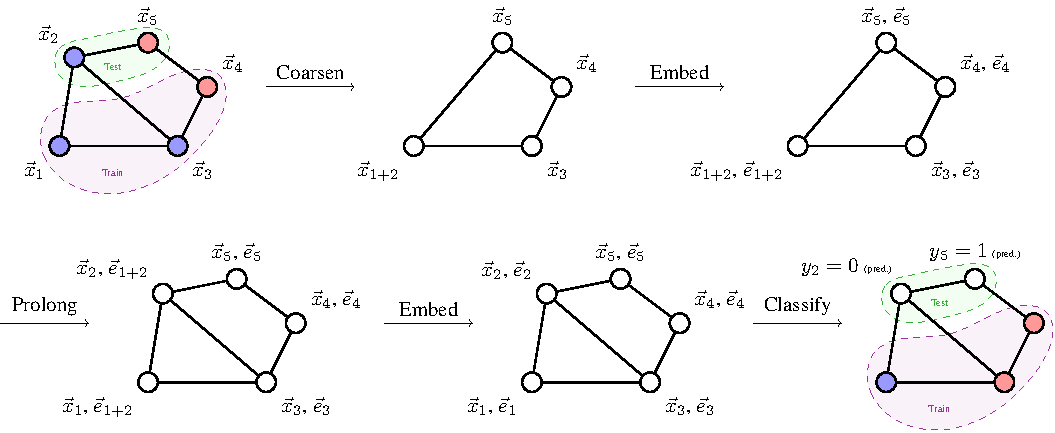
\includegraphics[width=\linewidth]{images/harp-overview/harp-overview.pdf}
  \caption{An overview of the HARP processing pipeline with one level of coarsening}
  \label{fig:harp-overview}
\end{figure}

\subsection{Balancing performance and complexity}

\todo{This is WIP and needs to be rewritten after next subsection is done}
Graph-based methods such as node2vec typically have a large number of parameters - on the widely used OGBN-ArXiv\todo{Don't mention OGB if no evaluation on OGB} dataset (see \cite{hu_open_2021}), the state-of-the-art node2vec model has over 21 million parameters. At the same time, recent works in the domain of graph learning have started to focus more heavily on simpler methods as a competitive alternative to heavy-weight ones (see \cite{frasca_sign_2020,huang_combining_2020,salha_keep_2019,zhang_eigen-gnn_2020}). As the authors of \cite{chen_harp_2018} observed, HARP improves the performance of models when fewer labelled data are available. The proposed lower complexity models based on HARP could also improve performance in a setting where only low fidelity data are available for large parts of the graph. Coarser models could be trained on them, with a subsequent training of finer models using only a limited sample of high fidelity data.

\subsection{Our method}
Explanation of the adaptive prolongation approach

\section{Experimental evaluation of the adaptive approach}
Show the results of the adaptive prolongation on multiple datasets, compare it to ordinary Node2vec and HARP.

Possibly include statistical significance testing.

\begin{figure}
  \centering
  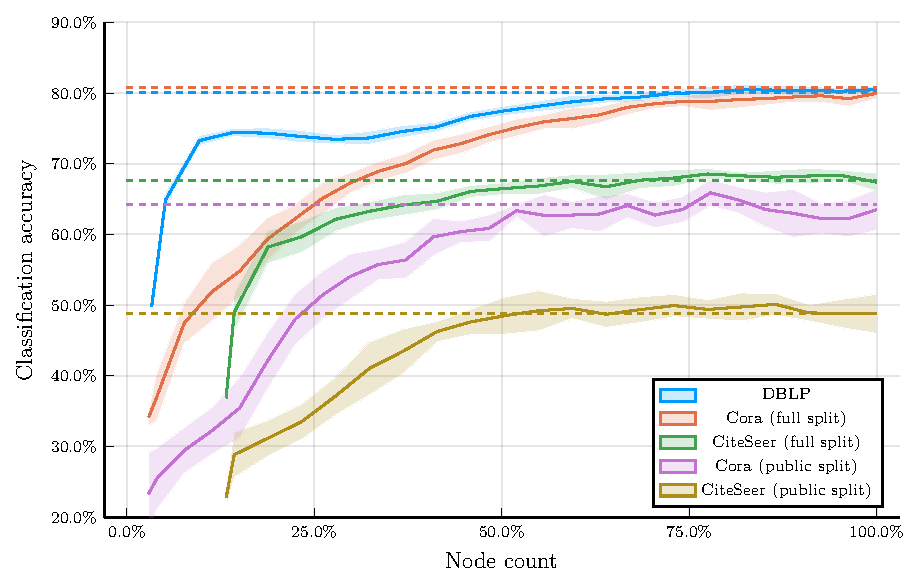
\includegraphics[width=\linewidth]{images/adaptive-coarsening/adaptive-coarsening.pdf}
  \caption{Adaptive coarsening results}
  \label{fig:adaptive-coarsening}
\end{figure}

\subsection{Relation to graph properties}

Compare the adaptive coarsening with local graph measures of graph homophilly

\section{More general approaches to coarsening}

\subsection{The PIHom framework}
Explain the general framework for coarsenings\todo{Only do this, if we can relate to it in any other parts of the paper}

\subsection{Graph diffusion coarsening}

\subsection{Evolved coarsening}

\section{Experimental comparison of coarsening approaches}

\section{Conclusion}

In our work in progress, a way to merge method generality, computational efficiency and high performance was explored. HARP and partially injective homomorphisms were presented and subsequently connected as a way to, in a future work, adapt graph coarsenings to a specific task. This connection was experimentally verified not to impact prediction performance. Furthermore, the effect of HARP pretraining on learning characteristics was studied and found to reduce the need for training on fine (and therefore large) graphs, making way for a more efficient training without sacrificing performance.


\begin{acknowledgments}
  The research reported in this paper has been supported by the Czech Science Foundation (GAČR) grant 18-18080S.
\end{acknowledgments}

\bibliography{zotero}

\end{document}
